\documentclass[english]{tktltiki}
\usepackage[pdftex]{graphicx}
\usepackage{subfigure}
\usepackage{url}
\begin{document}
%\doublespacing
%\singlespacing
\onehalfspacing

\title{Assignment 1: User research}
\author{P�ter Ivanics (pair: Julian Schulte)}
\date{\today}

\maketitle

\numberofpagesinformation{\numberofpages\ pages + \numberofappendixpages\ appendices}
\keywords{}

\mytableofcontents

\section{Introduction}
	This short report is a summary of a user research concerning the usage of tablet devices for reading and learning purposes. The report is rolled out as one of the assignment of the Human-Computer Interaction course and serves the purpose to gain hands-on experience with the course material. 
	
	The motivation behind choosing this topic mainly my own experience and interest, but also the common applicability of the problem. Personally, I never liked to read literature (novels, stories, poems etc.) from screen and preferred to use books instead. The main reason behind this is the fact that it felt more natural and less tired after finished reading. Nevertheless, individuals may have subjective opinions in this manner. For this reason, it would be interesting to see if others share the same feelings, why individuals prefer one or another way of reading. 
	
	There are plenty of researches ongoing in the present time about the potential replacement of textbooks with electronic devices in education. For example, several elementary and grammar schools started to hand over tablets to pupils instead of printed books in classroom environments. This has several positive outcomes, such as children do not have to carry heavy books with themselves day-by-day, teachers can present audiovisual material as part of the lessons to facilitate different styles of learning. Personally, I attempted to read study material and to add markup to my textbooks and lecture notes on a tablet, which I did not find convenient. Investigating this manner is another goal and motivation of this short study.
	
	This short research aims to discover the opinion of users concerning reading literature and study material from an iPad tablet. The research plan below describes the main guidelines and aspects that are utilized to conduct the research. Further, the findings are of a single person's interview session is described. Finally, some conclusions are made about my learning progress and gained experiences through this assignment both as interviewee and interviewer. 

\section{Research plan}

\subsection{Research questions}	

	As the first step of the research plan, the research question and its subquestions are formulated. The main research question is \textit{How does reading experience differ on a tabled compared to paper-based books?}  Due to the fact that this research question can have many aspects and may be too wide for this assignment, the scope is reduced to answer the following subquestions (and their methodological dimensions in parenthesis): 
	
	\begin{itemize}
		\item \textit{How does the reading experience of literature and coursebooks differ on tablets compared to paper-based books based on users' impressions?} (open-ended, interventionist, qualitative, subjective)
		\item \textit{Does it feel natural for readers to read from a tablet?} (close-ended, observational, quantitative, subjective)
		\item \textit{Do readers prefer books over tablets as sources of reading and study resources?} (close-ended, interventionist, quantitative, subjective)
		\item \textit{Do users find it difficult to use a tablet for studying (e.g. making markups, notes, bookmarks in a coursebook) more difficult compared to a regular coursebook?} (close-ended, interventionist, quantitative, subjective)
	\end{itemize}
	
	An in-depth research may include more aspects, such as efficiency/speed of reading, long-term reading and how it affects the reader eye's tiredness, focus and attention. As the assignment was targeting to practice the interview and observation methods, these are given for the study. Nevertheless, it is important to point out that some of the questions above can be answered through other qualitative and quantitative measures, e.g. surveys. In other words, different methods may be better choice to answer some of the questions above in a similar study. 
	
	\subsection{The interview structure}	
	
	To carry out the research, the following semi-structured interview plan is designed with the participant(s). To begin with, a 5-minute opening/introductory step is performed, where general information is told to the participant about the session. The aim of this is to make him/her comfortable and sure that he/she is motivated to participate in the study. These questions will also assist to establish trust throughout the interview.
	
	In the next 5 minutes, some background information is retrieved about the participant. It is important to ask simple and clear questions as below and let him/her express feelings and experiences. The collected information here aims to learn more about the participants, to discover their reading habits and technical background. This will make the participant relaxed as well as researchers may understand more details during the analysis.
	
	In the next 20-25 minutes, the participant is asked to perform some simple tasks. The interviewer should express and introduce the tasks with precision and make sure the participants understood what was asked. While performing the tasks, participants should not be hasted and put under pressure - they should be given time to perform the tasks and guidance, in case it is needed.
	
	Finally, the last 5 minutes is dedicated to close the interview. The participant is asked of his/her feelings, impressions and feedback. The interviewer should conclude the session and say thanks for the participation. 
	
	% where the interview is conducted
	Reading is a focused activity in general. The interviewee will be asked several questions during the session, noises and disturbances should be eliminated by carefully choosing the location. In order to achieve the best possible outcome, the interview should be conducted in a quiet environment. On the other hand, a laboratory room may not be a proper choice either, because it would make the participants feel uncomfortable. The best match probably would be a "living room"-like environment or a peaceful caf�, where the participants feel comfortable. 
	 
	% preparations/preconditions of the interview
	Prerequisites and preparation equipment for this interview includes the following:
	\begin{itemize}
		\item the tablet (e.g. iPad) which is going to be evaluated (make sure the battery is charged),
		\item a printed copy of literature (e.g. a novel),
		\item the PDF/ePub version of the same book downloaded to the device,
		\item any kind of university lecture slides (PDF/PPT) and a coursebook downloaded to the device,
		\item audio recorder (or camera) for recording the session,
		\item pen and paper for taking notes.
	\end{itemize}
	
	The next page lists the step-by-step schedule of the interview. The listed points are more guidelines than strict points to follow. Respect the time and leave points out if necessary. Let the participants finish their thoughts and do not interrupt their speech unless the discussion goes into deep details!
	
	\pagebreak
	\singlespacing
	\footnotesize
	
	\begin{itemize}
		\item \textbf{5 minutes: Opening}
		\begin{itemize}
			\item open the discussion,
			\item introduce the participant the content of the interview (what will happen),
			\item remind the participant that the interview will take approximately 40-45 minutes,
			\item ask the participant for permission about recording the session and ensure him/her that it will remain confidential material,
			\item ask the participant to introduce him/herself in couple of sentences,
			\item ask the participant how he/she feels,
			\item ask the participant if he/she has any questions before beginning the interview.
		\end{itemize}
		
		\item \textbf{5 minutes: Background information}
		\begin{itemize}
			\item ask how often does he/she read books,
			\item ask what kind of books are in his/her interest,
			\item ask if he/she prefers paper-based books rather than reading from electronic devices, 
			\item ask how familiar he/she is with mobile devices and tablets, 
			\item if the participant is not familiar with the device, give a short introduction about the usage.
		\end{itemize}
		
		\item \textbf{20-25 minutes: Tasks}
		\begin{enumerate}
			\item Literature reading (10 minutes)
			\begin{enumerate}
				\item open the book reader software (e.g. iBooks) and open a book of choice (a novel, a roman or similar literature) through the software,
			\item read 1-2 pages and express feelings (e.g. how does it feel to read from the screen, is it more difficult than from paper, does it feel natural to hold the device in hand in landscape and portrait orientation, etc.)
			\item give the same paper-based copy of a book to the participant; ask him/her to read 1-2 pages and express feelings in comparison to the previous experience (does this feel more natural, is the text easier or harder to read, etc.), 
			\end{enumerate}
			
			\item Study-related material (10 minutes)
			\begin{enumerate}
				\item open the book reader software (e.g. iBooks) and open a study related material (a coursebook or PPT lecture slides) through the software,
				\item browse through the pages and express feelings (how does it feel to read from the screen, is it more difficult than from paper, does it feel natural to hold the device in hand in landscape and portrait orientation, etc.)
				\item add couple of bookmarks to certain pages
				\item navigate between the added bookmarks, retrieve the saved pages, 
				\item add markups (own notes) to the contents of the material.
			\end{enumerate}
		\end{enumerate}
		
		\item \textbf{5 minutes: Closing, conclusions}
		\begin{itemize}
			\item close the discussion and summarize the interview,
			\item say thanks for participating in the study,
			\item if possible, provide small present,
			\item ask if there are any questions
		\end{itemize}
	\end{itemize}
	
	\pagebreak
	\normalsize
	\onehalfspacing

\section{Findings}
	With my pair we agreed to conduct the interview during one of the evenings in my apartment's living room. This is a cozy, familiar and peaceful environment for the interview with a lot of light, a sofa and small coffee table (\ref{}). All the required material and devices were prepared in advance of his arrival. When my pair has arrived I welcomed him with a tea and we had some casual discussion before getting started with the interview. 
	
	\begin{figure}[h] 
		\begin{center}
			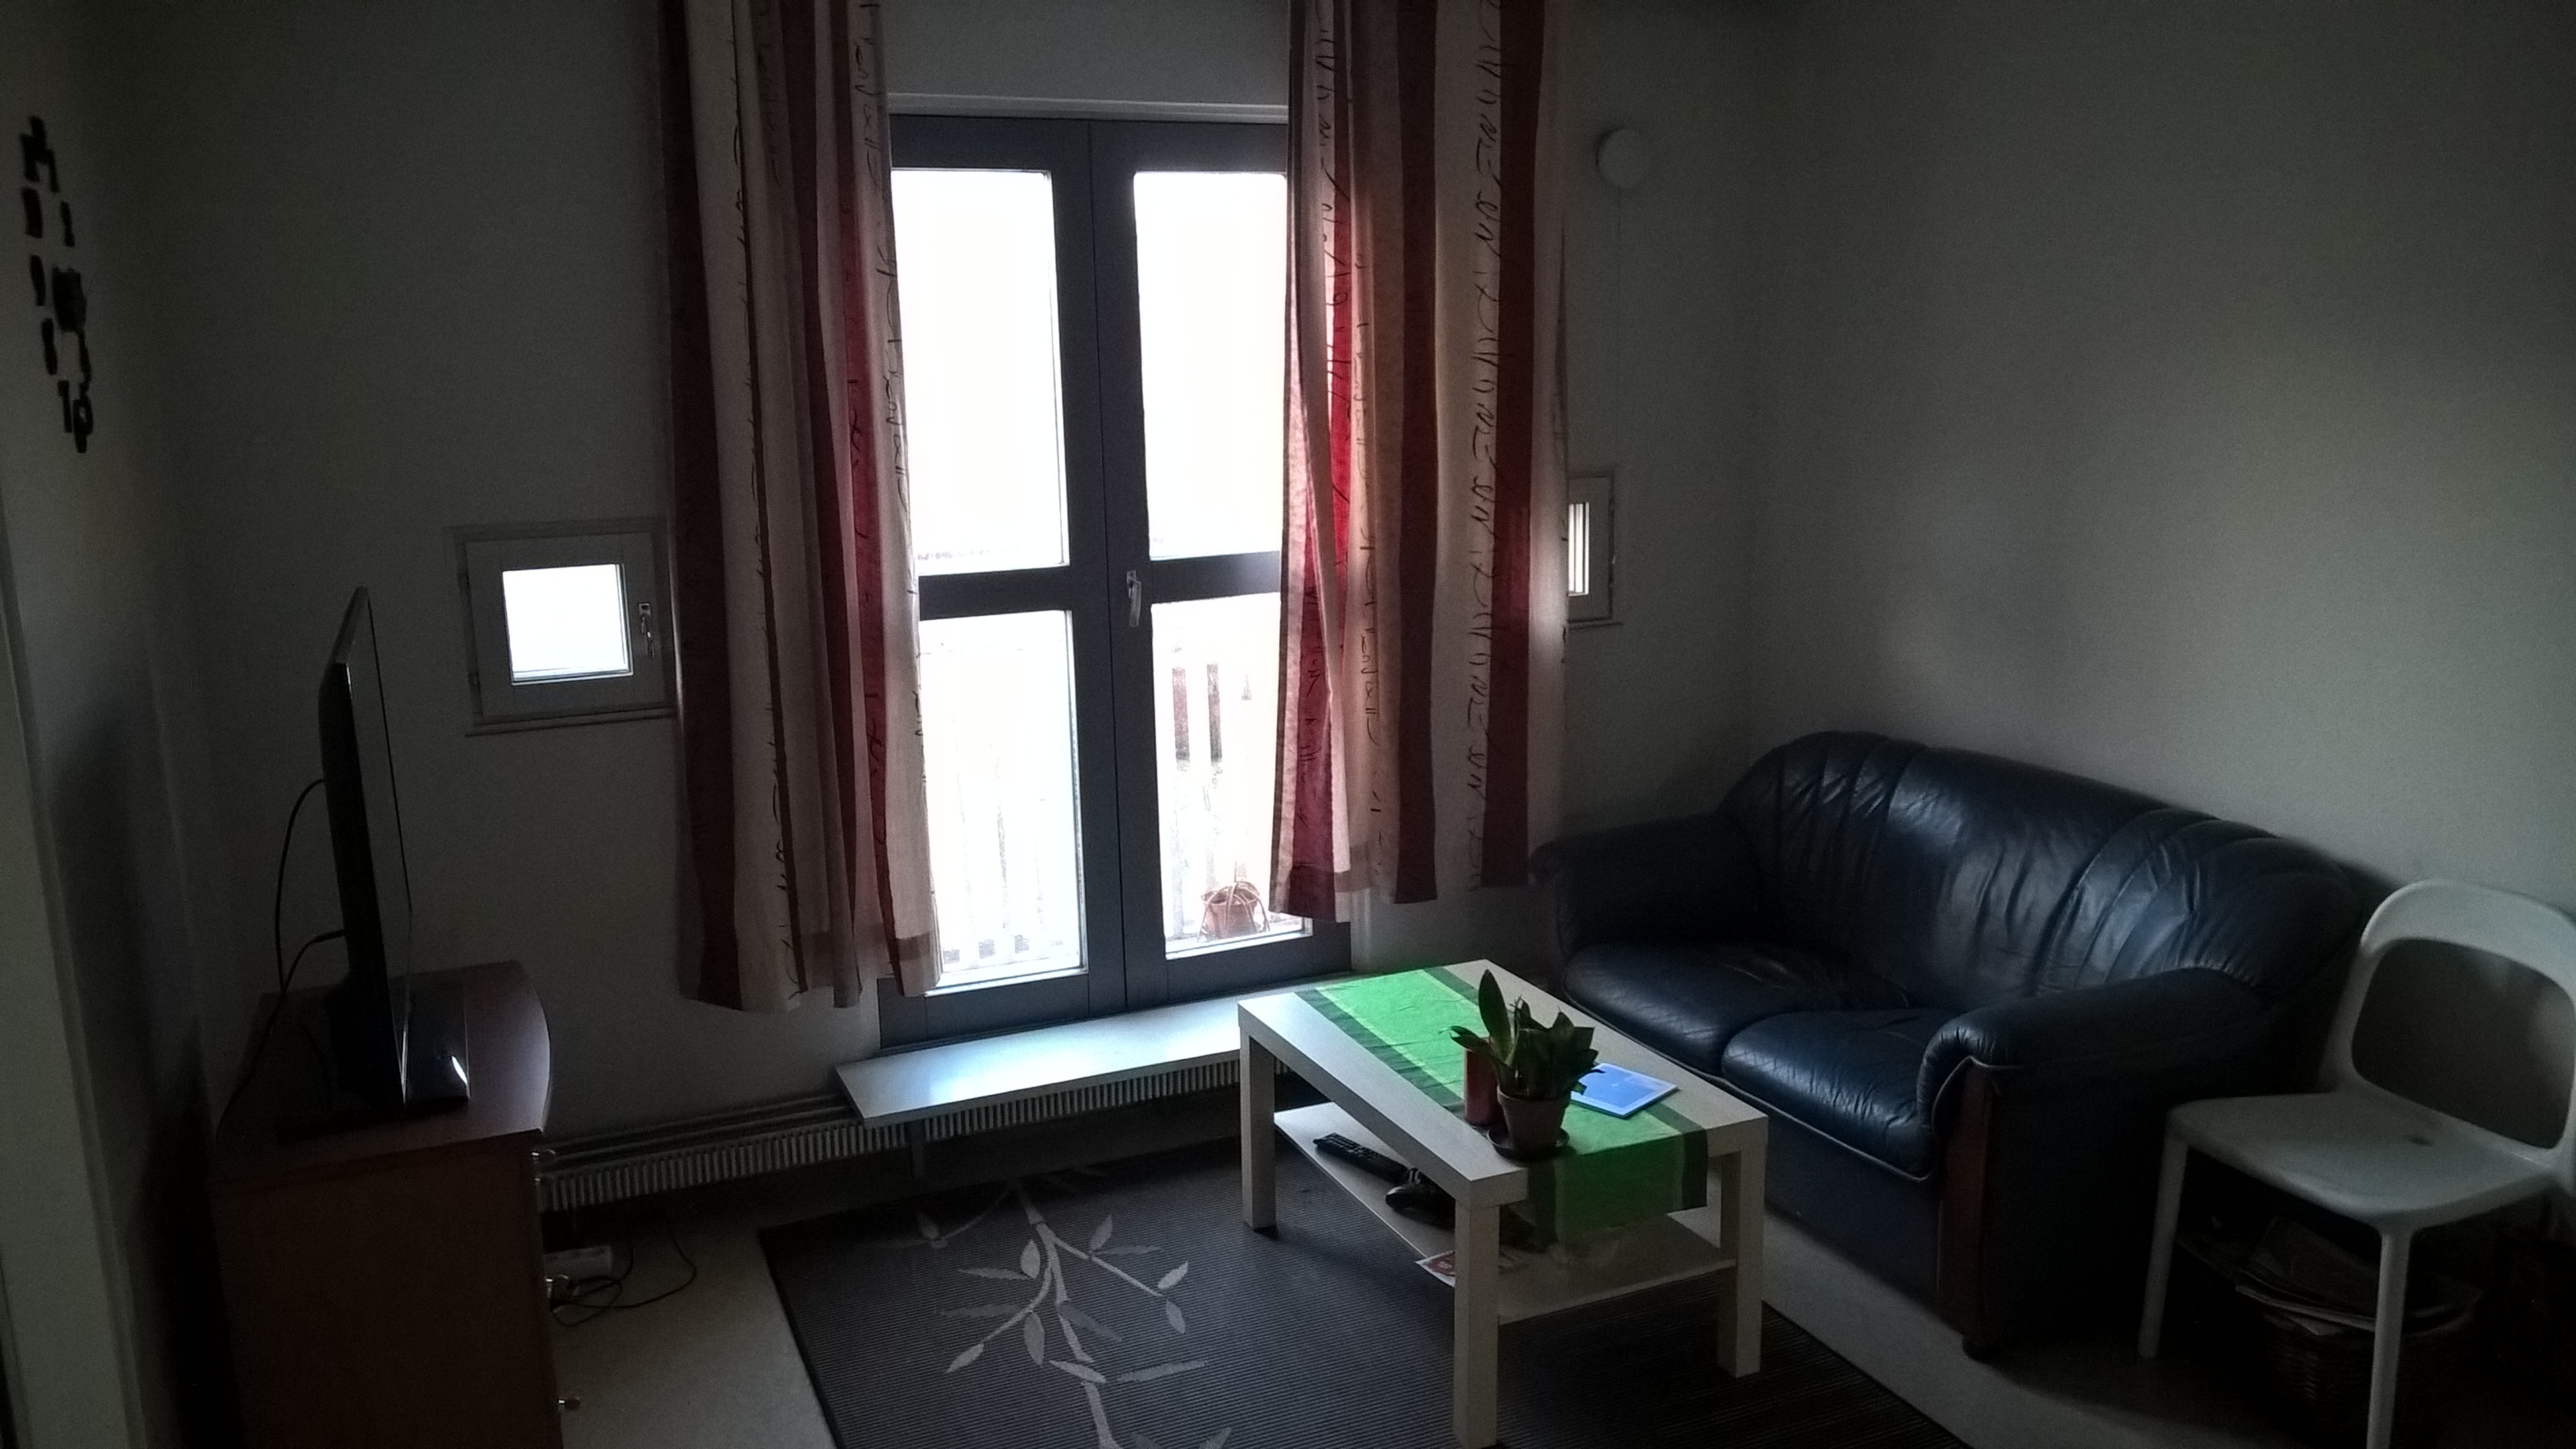
\includegraphics[height=0.4\textwidth]{images/living-room.jpg}
			\caption{The environment where the interview was conducted.}
			\label{living-room}
		\end{center}
	\end{figure}
	
	In the opening of the interview, I payed careful attention to introduce the context and the setting to my pair and asked if the session's audio can be recorded. I explained the structure and the timing of the interview briefly. I learned about my pair, that he is an exchange student from Germany, studies computer science on bachelor level. 
	
	Next, I asked some of the background information, including his current reading habits and usage of mobile devices. He explained that recently he was not reading books actively, but previously he used to read a lot of novels, fantasy stories, criminal books, comics, manga or as he expressed "pretty much everything". On top of that, he reads study-related material (coursebooks and PDF slides) on a regular basis as a university student. He turned out to be a regular smart phone user with different purposes: calling, chatting, surfing on the internet and playing games. However, he clearly expressed his unfamiliarity with tablets and the fact that he is not a regular user. In addition, it was said "I prefer reading books in actual paper form, whilst as lecture slides are mostly available online, I tend to read them from my personal computer". Finally, he stated that because the computer screen is bigger than a tablet, he prefers to study lecture slides through this media. 
	
	After introducing the first task I gave the tablet to my pair. At first he was not sure how to unlock the screen of the device and open the eBook reader application (iBooks), however he figured it out very quickly without guidance. He managed to start using the device and to find and open the book I asked for. This allows drawing the conclusion that the device is intuitive to use and easy to get started with. 
	
	I asked him to read couple of pages from the tablet and gave approximately 2-3 minutes of silence for focusing on the content. Meanwhile he was reading the novel (J.K. Rowling - Harry Potter and the Prisoner of Azkaban), I was observing his motions and expressions. He seemed to act naturally, he did not face any major problems with navigating between the pages or reading from the screen. 

	Next, I asked how does he feel to read the book from the screen at first. He replied "It is hard to describe. It is not bad to read, but it is definitely different compared to a real book (...) My main issue is the size and the shape of the tablet is different compared to a book". This allows to derive the fact that the reading experience is strongly influenced by the fact that the weight and the shape of the device is not the same as a book. The reader subconsciously expects paper to be in his hands, however the exterior surface and the weight of the tablet creates a different experience. 
	
	"Navigating between the pages is natural", as expressed by my pair. He says that since he is familiar with smart devices and technology, he can easily get used to the swipe gesture which simulates the motion of turning a page in a book. He also noticed that tapping once on the left or right side of the screen navigates backwards and forwards in the book. He could easily figure out how to use the controls to navigate multiple pages forwards and backwards in the book (Figure \ref{book-screenshot}). This allows to conclude that the navigation is intuitive for a technical person, nevertheless it would be interesting to see how less technical-oriented users would feel about this manner. 
	
	\begin{figure}[h] 
		\begin{center}
			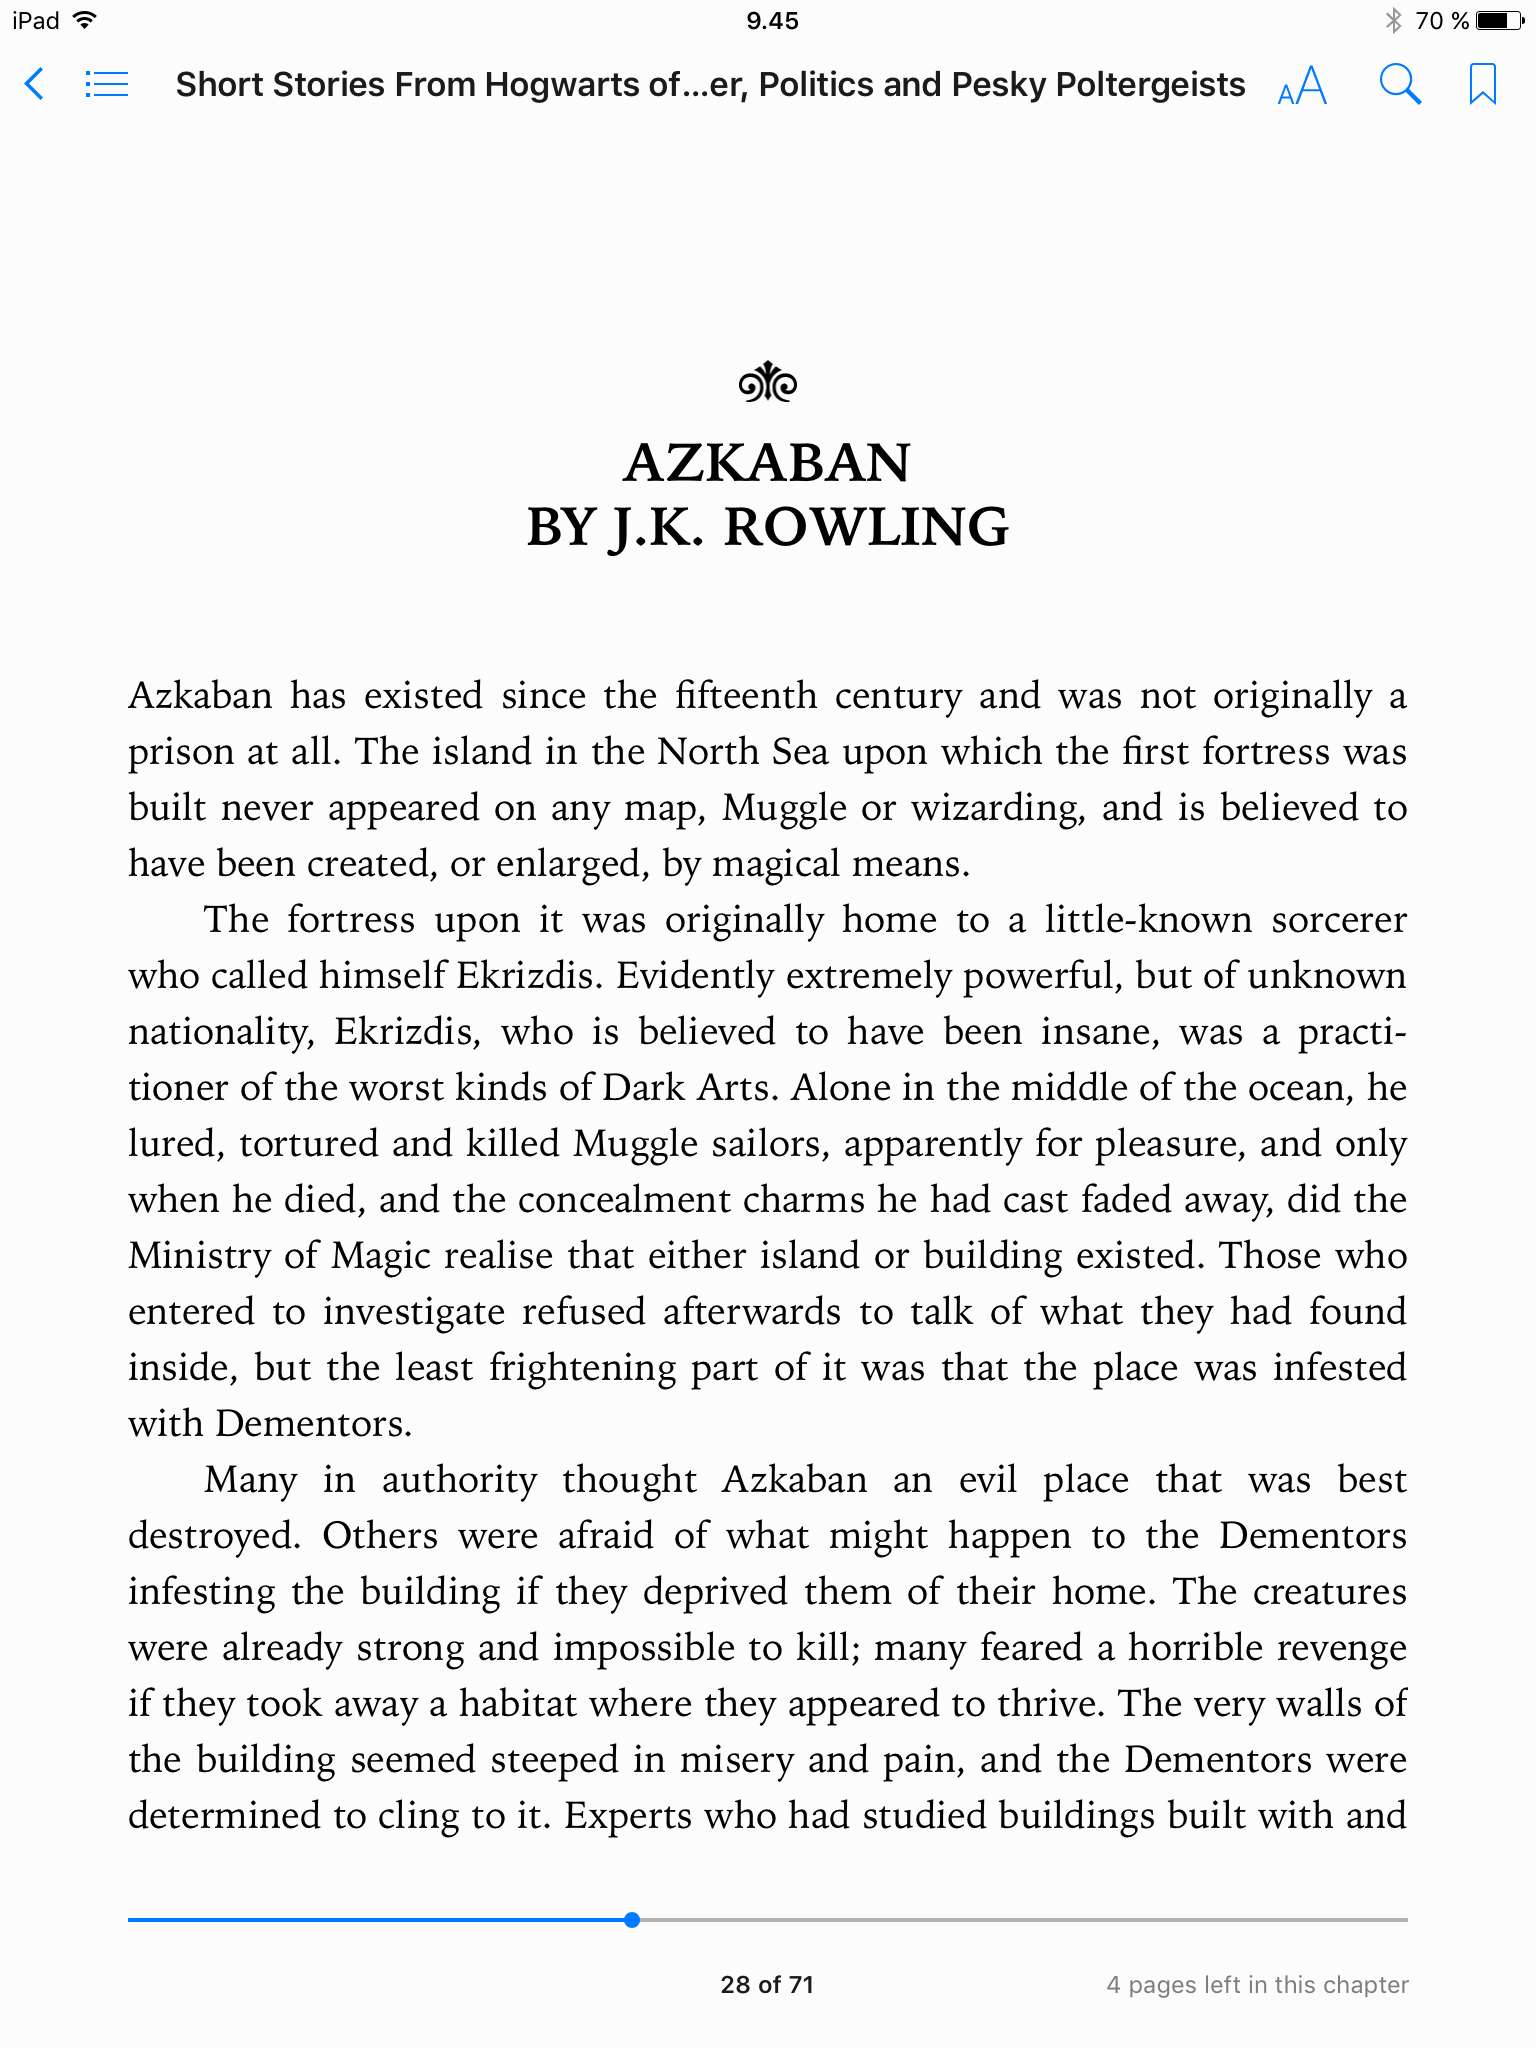
\includegraphics[height=0.75\textwidth]{images/IMG_0031.PNG}
			\caption{A screenshot from the tablet while reading a book. On the top of the screen some indicator controls, on the bottom of the screen the navigation slider control is displayed.}
			\label{book-screenshot}
		\end{center}
	\end{figure}
	
	One important finding on the tablet was that there are a lot of distracting controls on the top of the screen (Figure \ref{book-screenshot}), for instance the battery status, time, wireless signal strength etc. On top of that, some other applications might make notifications appear on the screen which further disrupts the reader from focusing on the book's content. As he explained "for me on the long run this would be probably disturbing, because I get easily disrupted in my peripheral vision. If something pops up or blinks on the edge of the screen (...) I get easily disrupted". 
	
	After handing actual the book to my pair, he immediately said he was more "sucked" into the content of the book. He said he had to focus on the pages more as they were a bit yellow and the content was not supported that much with light. He explained "I had to focus on the content more because there was less light".
	
	Reading experience for study material/coursebooks differs even more than regular literature. My pair explained that the highlighted terms in a coursebook (Peter Flach - Machine Learning: The Art and Science of Algorithms that Make Sense of Data) are much more easier to identify if he is scanning for a particular piece of text on the tablet. This is because the emphasis on the different font styles and sizes on the screen are much more visible than on paper. He said "on the tabled every color is clearly visible, (...) while in the book the bold-phased text does not stand out that much". We concluded that the tablet facilitates learning in this context, because highlighted keywords, formulas, variables might are easier to find on the tablet compared to the book (Figure \ref{coursebook-screenshot}). 
	
	\begin{figure}[h] 
		\begin{center}
			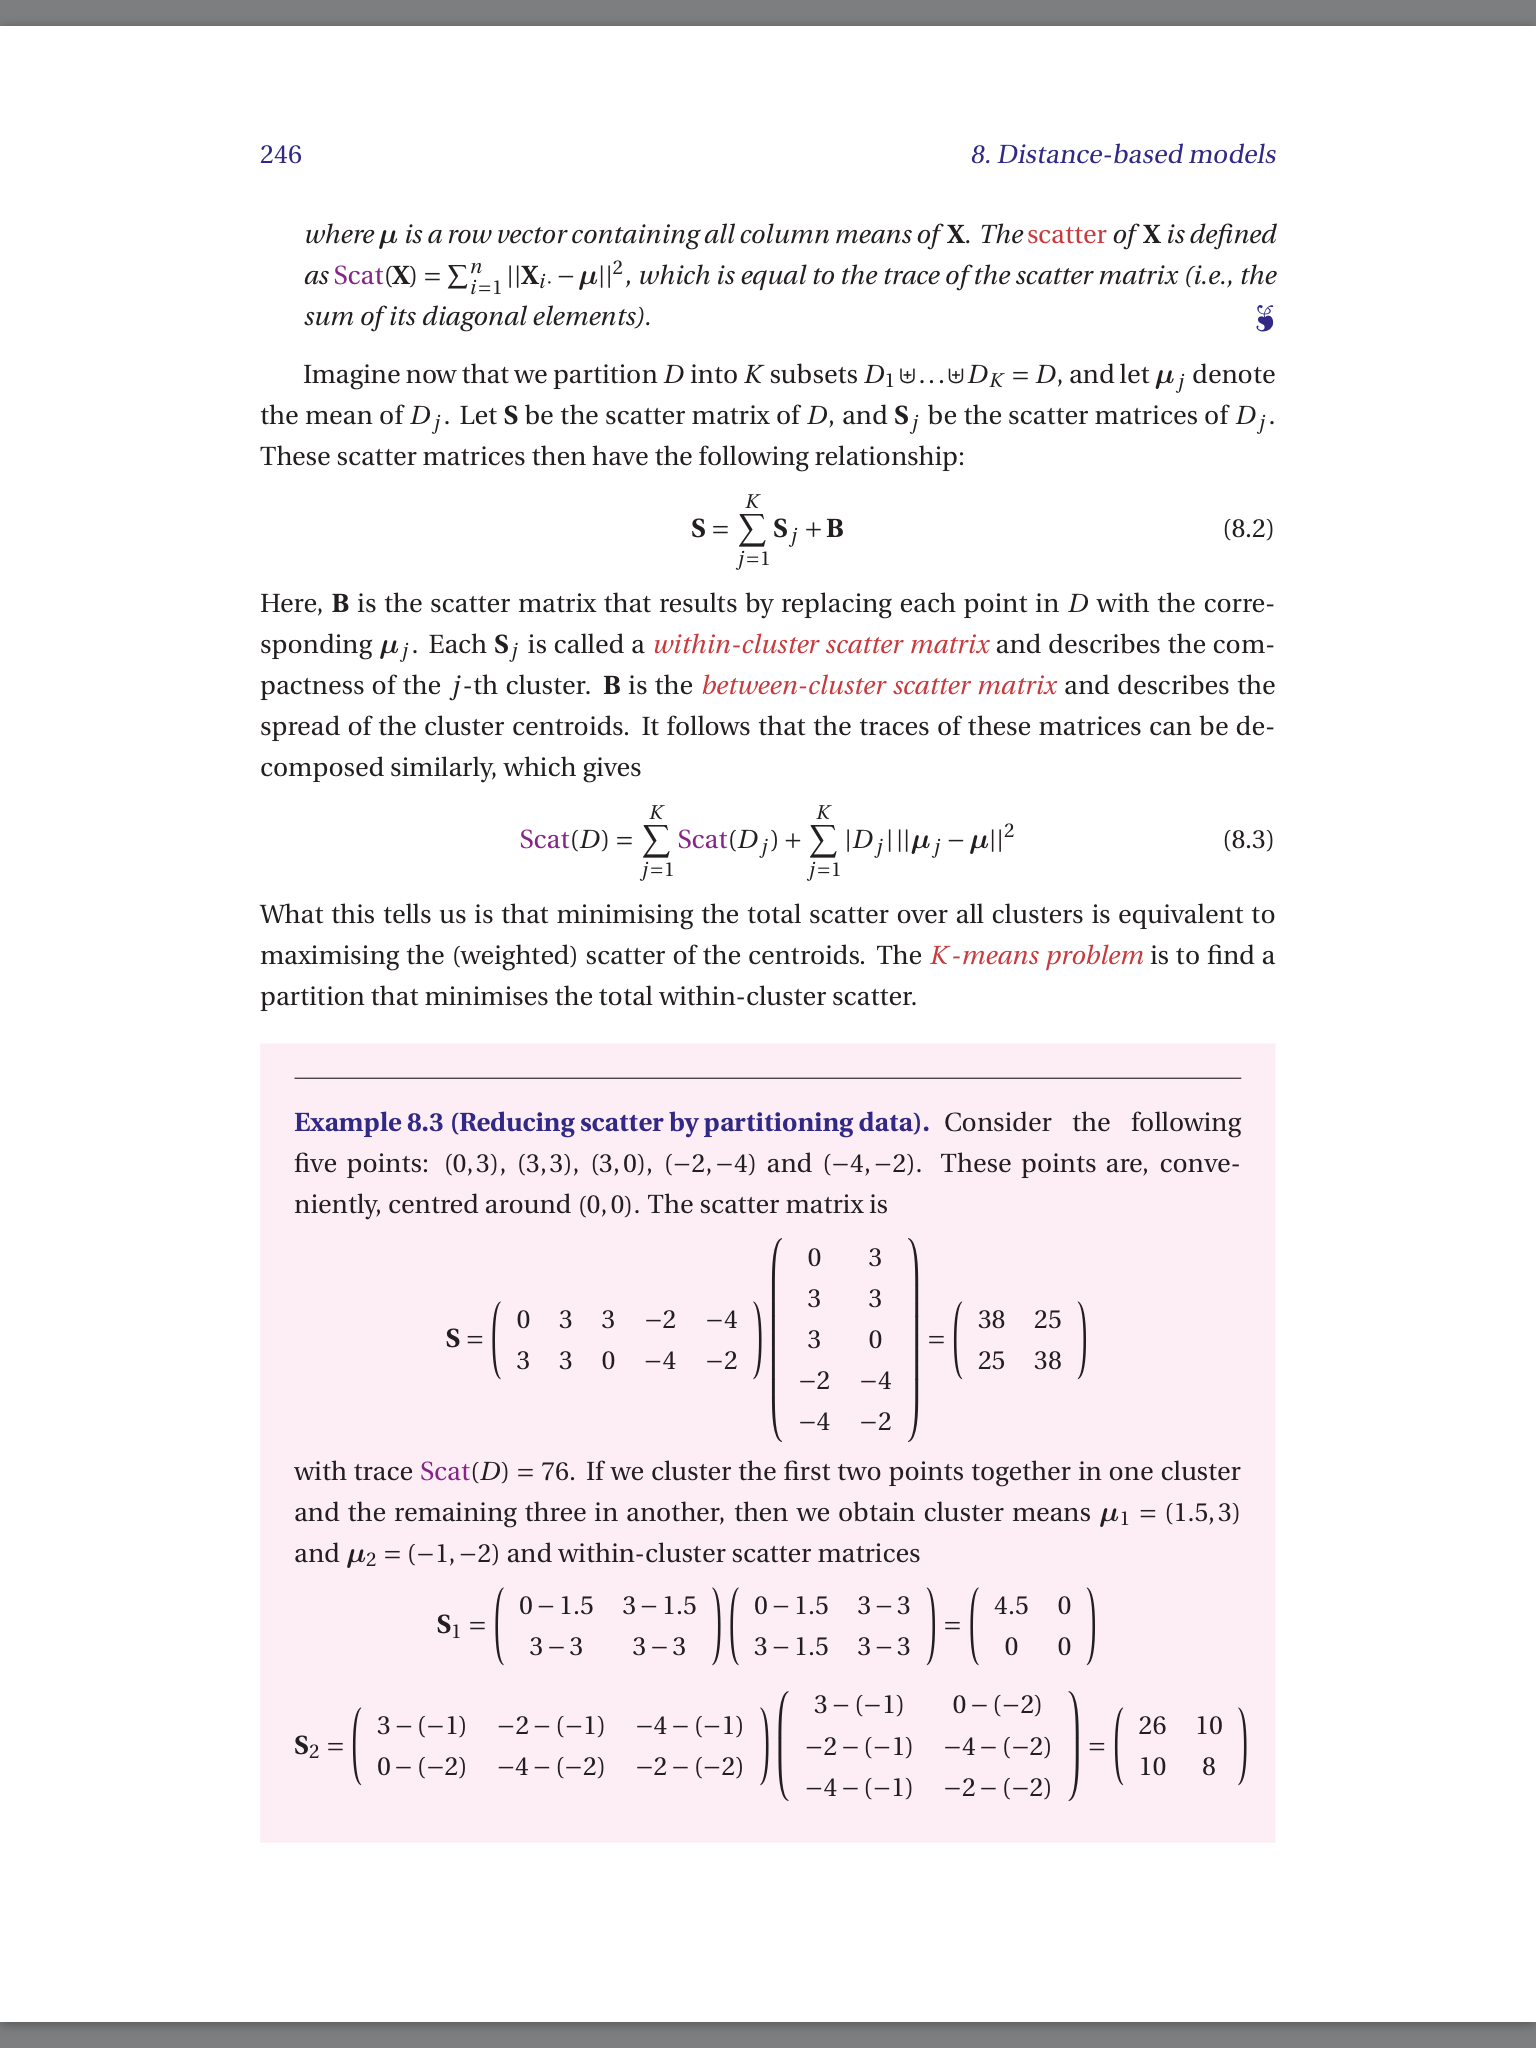
\includegraphics[height=0.75\textwidth]{images/IMG_0030.PNG}
			\caption{A screenshot from the tablet while reading a coursebook. The bold-phased keywords and keywords are nicely visible on the actual screen of the device and support scanning better than on paper.}
			\label{coursebook-screenshot}
		\end{center}
	\end{figure}
	
	Last but not least, I asked my pair to add some bookmarks to the coursebook and retrieve them on the tablet. He could find the way to retrieve the bookmarks without major problems. However, he could not clearly make distinction between the content of the bookmarked pages based on the preview displayed on the screen. In other words, it was a bit difficult to recognize which bookmark points to which part of the book and what the content will be after opening them. In comparison, he said that printed coursebooks are bookmarked by colorful sticky notes or labels by many students. We discussed that the latter is an easier way to handle bookmarks and may be more efficient way of marking important pages of a coursebook.
	
\section{Conclusions}

	In my opinion the preliminary research plan matched the research questions and identified a lot of findings. The interview was carried out successfully and greatly contributed to the study. Nevertheless, as the interview was done with only one person, it would be interesting to repeat a similar session with other participants - especially with someone who comes from a different age group and background. 

	The interview plan was followed successfully. The scheduled five minutes for this section was filled, we completed the interview in around 40 minutes. However, the Opening and the background information section took only 5 minutes altogether and we spent a bit more time with the tasks after all. Accordingly, the schedule could be corrected at this point. The tasks took approximately 10 minutes each and the closing went also according to the schedule. 
	
	After the interview I noticed that some of the tasks were missed (e.g. trying to add markups to the coursebook). Nevertheless, the time was filled and a lot of findings were identified. I believe, the location was chosen well for this session, however at some point my flatmate arrived home which slightly disturbed the session. Next time I could pay more attention to such details. In sum, I really enjoyed carrying out such interview and I was surprised about some of the findings as they were unexpected. 
	
	Being a participant was a very interesting experience as well. We conducted the interview the other way around on the following day in the same living room. I could put my focus on the task and got carried away with the flow of the interview. I think my pair planned well ahead as he had all the required material and tasks prepared very well for me. Both of us had a positive outcome and impression on the task as a interviewee and interviewer as well. 
	
\pagebreak
\nocite{*}
\bibliographystyle{tktl}
\bibliography{bibliography}

\lastpage

\end{document}